\documentclass[11pt,a4paper,oneside]{article}
\usepackage[latin1]{inputenc}
\usepackage{amsmath}
\usepackage{amsfonts}
\usepackage{amssymb}
\usepackage{graphicx}
\usepackage{color}
\usepackage {tikz}
\usepackage{fancyvrb}
\usetikzlibrary {er}
\usepackage[left=2.00cm, right=2.00cm, top=1.00cm]{geometry}
\graphicspath{{./}}
\fvset{tabsize=4}

\begin{document}
	\title{DS 255 - System Virtualization \\ Assignment I - OS Primer}
	\author{Shriram R. \\ M Tech (CDS) \\ 06-02-01-10-51-18-1-15763}
	\maketitle	
	
	\begin{enumerate}
		\item Modern ISAs like Intel x86 support four different execution privileges or protection rings with one for OS Kernel, two for OS Services and one for the Applications. OS Kernel has the highest privilege while the Application will have the lowest privilege. This is illustrated in the figure given below,
		      \begin{center}
		         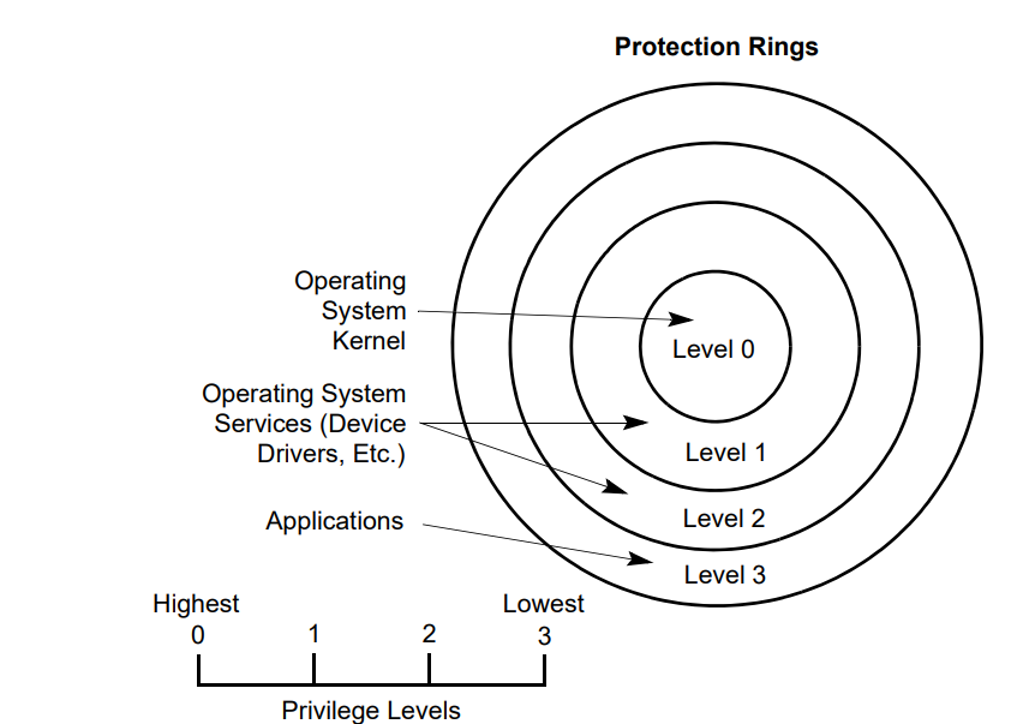
\includegraphics[scale=0.4]{1.png}		
		      \end{center}
		These privileges are necessary to enable the OS to establish control over the system and restrict user processes from gaining arbitrary access to more resources or memory space of other processes. Modern Operating systems typically support Level 0 (Kernel) and Level 1 (User) execution modes. \\
		
		For x86, the current mode of execution can be determined by examining the lower two-bits set in code segment register. This should be similar in the other architectures as well. \\
		
		A proess can change its privilege from user mode to kernel mode by making a system call. Note that a process cannot execute arbitray instructions of its own during kernel mode. The following happens when a system call is made,
		\begin{enumerate}
			\item Process registers are saved to kernel stack and mode is changed to kernel mode
			\item OS trap handler performs execution of its code in kernel mode
			\item After trap handler completes execution, process registers are restored from the process stack and mode is changed to user mode
			\item Process continues execution in user mode   
		\end{enumerate} 
	   
	    \begin{verbatim}
	    
	    \end{verbatim}
	
		
		\item
		\item	
		\item		
		%\begin{center}
		%	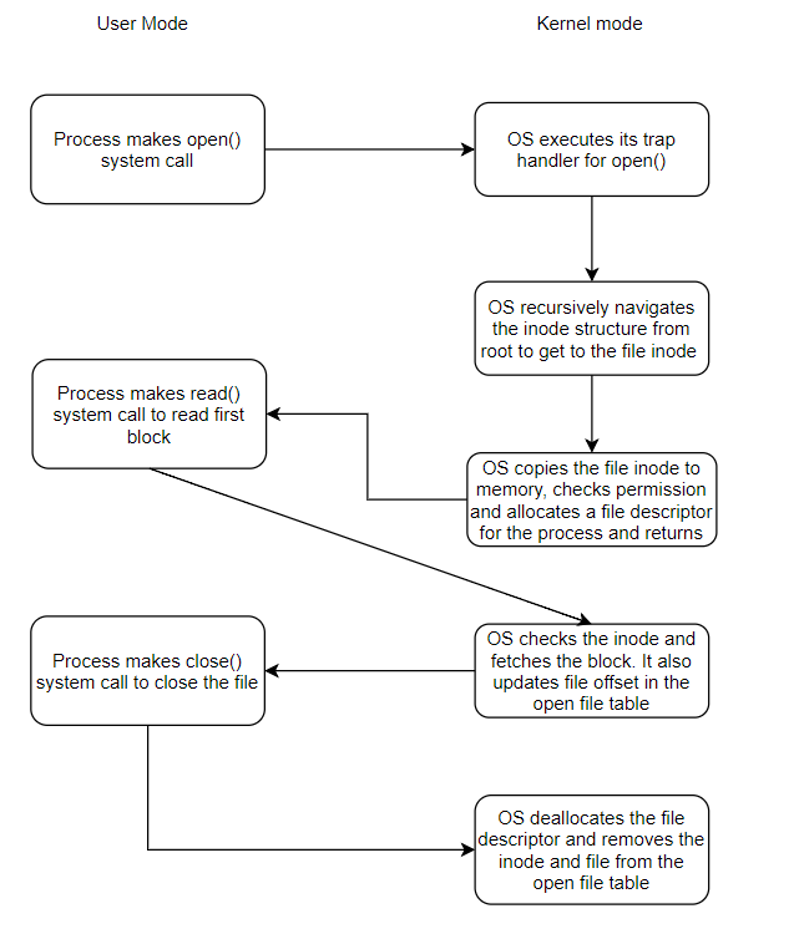
\includegraphics[scale=1.0]{3.png}		
		%\end{center}		
				
	\end{enumerate}
    
	
	  \begin{center}
		%\begin{tabular}{|c|c|c|c|}
			%\hline 
			%\textbf{Processes}  & \textbf{Sequential (Avg.) (s)} & \textbf{Parallel (Avg.) (s)} & \textbf{Speedup} \\
			%\hline
			%2 &  0.0311 & 0.0165 & 1.88\\ 
			%\hline
			%4 &  0.0311 & 0.0096 & 3.22\\ 
			%\hline
		%\end{tabular}
	\end{center}
    
    \section{References}
    \begin{enumerate}
    	\item Intel\textsuperscript{�} 64 and IA-32 Architectures Software Developer's Manual Combined Volumes: 1, 2A, 2B, 2C, 2D, 3A, 3B, 3C, 3D, and 4
    	\item Operating Systems: Three Easy Pieces, Remzi H. Arpaci-Dusseau and Andrea C. Arpaci-Dusseau, Arpaci-Dusseau Books.
    \end{enumerate}
 

    
\end{document}